\section{Proposed system}
	\subsection{Overview}
	\subsection{Functional Requirements}
	\subsection{Nonfunctional Requirements}				%3_03
		\subsubsection*{}
		{\tabulinesep=1.2mm
\begin{tabu}{ | p{3cm} | p{13cm} |}
    \hline
    Category	 			& 		Requirements \\\hline
    Usability:	  			& 		98\% of the 15-30-year-olds users should be able create, delete, edit appointments and account without prior knowledge, reading or education. \\\hline
    Reliability: 			& 		- Crashes/loss of connection must not cause loss of neither account- or appointment information, none-submitted data may be lost. \\
							&		- It should always be possible to access the server, when the client has Internet connection.\\
							&		- Crashes should be rare - less than 1\% of operations made by a user may lead to a crash. \\ \hline
	Performance:			&		- The system should be scalable - there should only be a hardware limit to the number of appointments or accounts in the system.\\
							&		- The calendar should load fast - there should be a maximum 1-2 second delay on normal computers with 1 mbit connection.\\
							&		- Client should be able to run on a single core 500 MHz CPU.\\ \hline
    Supportability: 		& 		- The system should be documented.  \\
    						&		- Update-able to new browsers and OS'. \\ \hline
	Implementation: 		&		- Requires an Internet connection.\\\hline
	Operation:				&	 	- None. \\\hline
	Legal:					&		- User should agree to terms of use.\\\hline
\end{tabu}
}
\\
	\subsection{System models}							%3_04
		\subsubsection{Scenarios}
			\paragraph{Scenario 1: Create Appointment:}
			 -\\
				\makebox{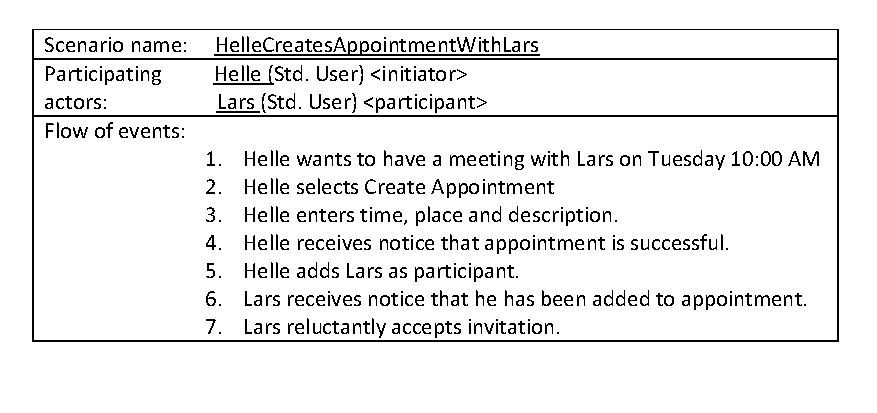
\includegraphics[scale=0.8]{docs/ScCreateApt.pdf}}

			\paragraph{Scenario 2: Create User:}
			 -\\
				\makebox{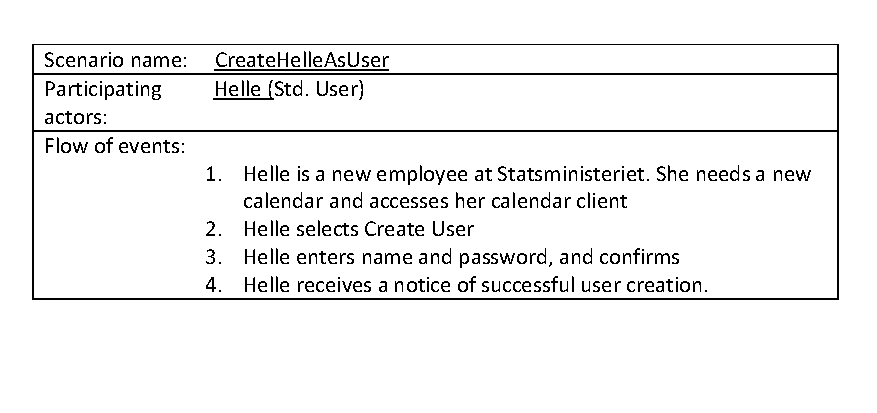
\includegraphics[scale=0.8]{docs/ScCreateUser.pdf}}
			
			Note: We need to figure out how to handle user-relationsship. 
			It is unlikely everybody able to invite all users. Do we have user-friendship, groups.. etc?

		\subsubsection{Use case model}
			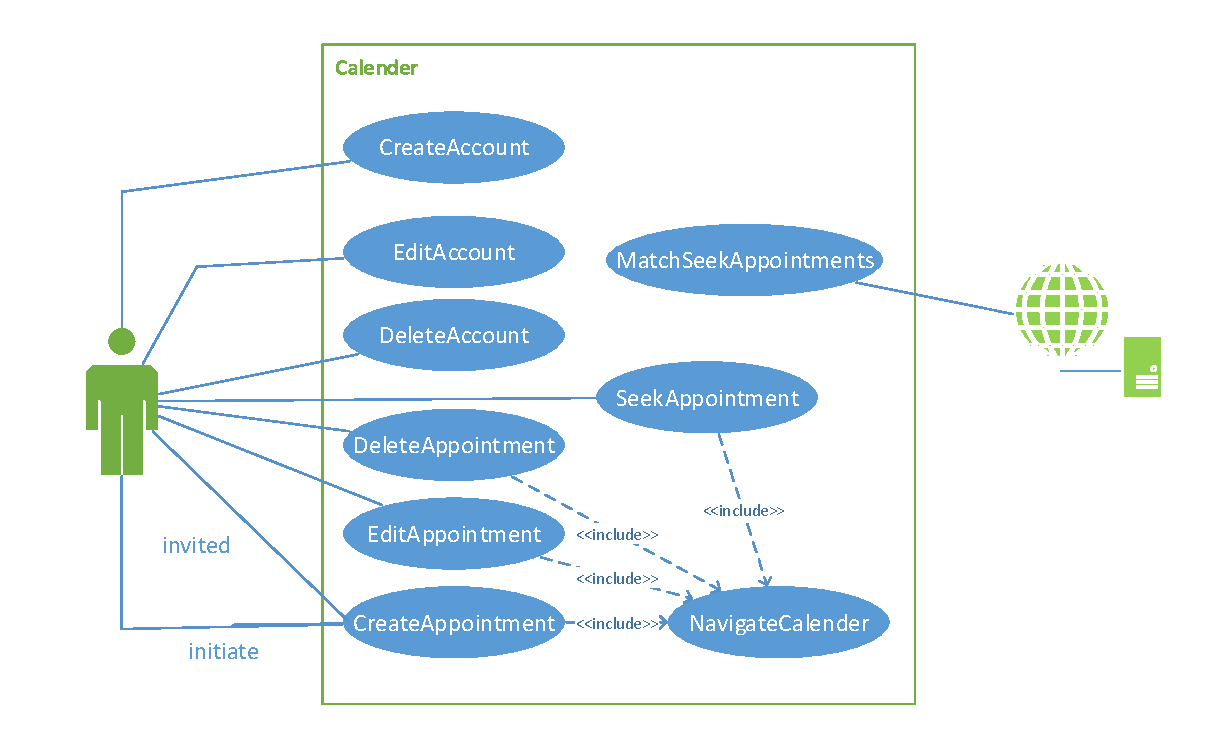
\includepdf[scale=0.7]{docs/UMLUsecaseDiagramCALENDAR.pdf}
			\begin{center}	
				{\tabulinesep=1.2mm
\begin{tabu}{ | p{3cm} | p{13cm} |}
    \hline
    Use case name: 			& 		CreateAppointment\\ \hline
    Participating  			& 		User wants to create an appointment with some friends and seeks additional participants. \\
    actors:					&		Users invited to the appointment.\\ \hline
    Flow of events: 		& 		1. User opens Calendar. \\
							&		2. Calendar shows the calendar navigation.\\
							&		3. User selects the date and time of the appointment.\\
							&		4. Calendar shows a form for entering description and place and participants.\\
							&		5. User fills the form, adds participants through email and enters how many additional participants he seeks.\\
							&		6. Calendar creates the appointment and notify participants that they have been added to the event.\\
							&		7. Her er en øndring i denne usacase.\\ \hline
    Entry condition: 		& 		- User is logged in  \\ \hline
	Exit conditions: 		&		- Appointment is changed.\\
							&		- User close the system.\\
							&		- Connection lost.\\\hline
	Quality requirements	&	 	- None \\\hline
\end{tabu}
}\\
				{\tabulinesep=1.2mm
\begin{tabu}{ | p{3cm} | p{13cm} |}
    \hline
    Use case name: 			& 		EditAppointment\\ \hline
    Participating  			& 		User wants to edit time and date of an appointment. \\
    actors:					& 		\\ \hline
    Flow of events: 		& 		1. User opens Calender. \\
							&		2. Calender shows the calender navigation.\\
							&		3. User selects the appointment he wants to change.\\
							&		4. Calender shows the appointment in normal mode that allows changes.\\
							&		5. User enters submits the wished changes.\\
							&		6. Calender updates the appointment and notify potential participants about the changes.\\ \hline
    Entry condition: 		& 		- User is logged in  \\ \hline
	Exit conditions: 		&		- Appointment is changed.\\
							&		- User close the system.\\
							&		- Connection lost.\\\hline
	Quality requirements	&	 	- None \\\hline
\end{tabu}
}\\
				{\tabulinesep=1.2mm
\begin{tabu}{ | p{3cm} | p{13cm} |}
    \hline
    Use case name: 			& 		DeleteAccount\\ \hline
    Participating  			& 		User wants to delete her account. \\
    actors:					&		Other users effected by deletion.\\ \hline
    Flow of events: 		& 		1. User opens the program. \\
							&		2. Calendar shows the calendar navigation.\\
							&		3. User selects edit profile.\\
							&		4. Calendar shows the profile edit.\\
							&		5. User select delete account.\\
							&		6. Calendar removes the user from all appointment. If the user was the only participant, the appointment is deleted.\\
							&		7. Calendar deletes account, and notifies other users about changes made to their appointments. \\\hline
    Entry condition: 		& 		- User is logged in  \\ \hline
	Exit conditions: 		&		- User account is deleted.\\
							&		- User close the system.\\
							&		- Connection lost.\\\hline
	Quality requirements	&	 	- None \\\hline
\end{tabu}
}\\
				{\tabulinesep=1.2mm
\begin{tabu}{ | p{3cm} | p{13cm} |}
    \hline
    Use case name: 			& 		DeleteAppointment\\ \hline
    Participating  			& 		User wants to delete an appointment. \\
    actors:					&		Other users effected by deletion.\\ \hline
    Flow of events: 		& 		1. User opens LuckyCalendar. \\
							&		2. LuckyCalendar shows the calendar navigation.\\
							&		3. User selects the appointment he wants to delete.\\
							&		4. LuckyCalendar shows the appointment in normal mode that allows changes.\\
							&		5. User selects delete appointment the wished changes.\\
							&		6. LuckyCalendar changes/deletes the event accordingly and notify other participants.\\\hline
    Entry condition: 		& 		- User is logged in.  \\ \hline
	Exit conditions: 		&		- Appointment is deleted.\\
							&		- User closes the system.\\
							&		- Connection lost.\\\hline
	Quality requirements	&	 	- None \\\hline
\end{tabu}
}\\
				{\tabulinesep=1.2mm
\begin{tabu}{ | p{3cm} | p{13cm} |}
    \hline
    Use case name: 			& 		MatchAppointments\\ \hline
    Participating actors:	& 		Calendar is matching appointments missing people with with people seeking appointment. \\
 							&		Users seeking appointment and users looking for appoitnment.\\ \hline
    Flow of events: 		& 		1. Calendar finds all appointments looking for participants. \\
							&		2. For each missing participant Calendar searches for a person seeking an appointment.\\
							&		3. If a match is found, the person is added to the appointment.\\
							&		4. Calendar notifies all users added to an appointment, and user who have an appointment where users are added to. User and appointments where no matches has been found, are notified if they are within a certain timelimit of the appointment.\\\hline
    Entry condition: 		& 		- Calendar runs this procedure x times a day. \\ \hline
	Exit conditions: 		&		- Calendar has looked through all apppointments.\\\hline
	Quality requirements	&	 	- None \\\hline
	Notes					&	 	- We might need a more clever approach, if we as many people getting an appointment as possible \\\hline
\end{tabu}
}\\
			\end{center}
		\subsubsection{Object model}
		\subsubsection{Dynamic model}
		\subsubsection{User interface}